% D1.2-style interim report for Sketch-Vision
\documentclass[11pt,a4paper]{article}
\usepackage[margin=1in]{geometry}
\usepackage[utf8]{inputenc}
\usepackage[T1]{fontenc}
\usepackage{graphicx}
\usepackage{hyperref}
\usepackage{booktabs}
\usepackage{enumitem}
\hypersetup{colorlinks=true, linkcolor=black, urlcolor=blue, citecolor=black}

\title{Sketch-Vision: Primitive Detection and Program Reconstruction\\\large D1.2 Progress Report}
\author{Team JAXAXAX\\Nikita Zagainov, Nikita Tsukanov, Said Kadirov, Dmitry Tetkin}
\date{\today}

\begin{document}
\maketitle

\begin{abstract}
We extend raster-to-program modeling to hand-drawn sketches with engineering annotations. This interim deliverable documents (i) a lightweight synthetic dataset generator with JSON annotations, (ii) visualization and evaluation utilities, and (iii) updated repository documentation. We outline alignment with CAD2Program-style VLMs and next steps.
\end{abstract}

\section{Overview}
Our goal is to detect digits, arrows, dimensions, radii, and geometric primitives in noisy sketches, producing a structured representation suitable for downstream CAD. We follow the encoder--decoder paradigm (ViT encoder + LM decoder) summarized in our prior notes (see `docs/sketch-vision-eng.pdf`).

\begin{figure}[h]
  \centering
  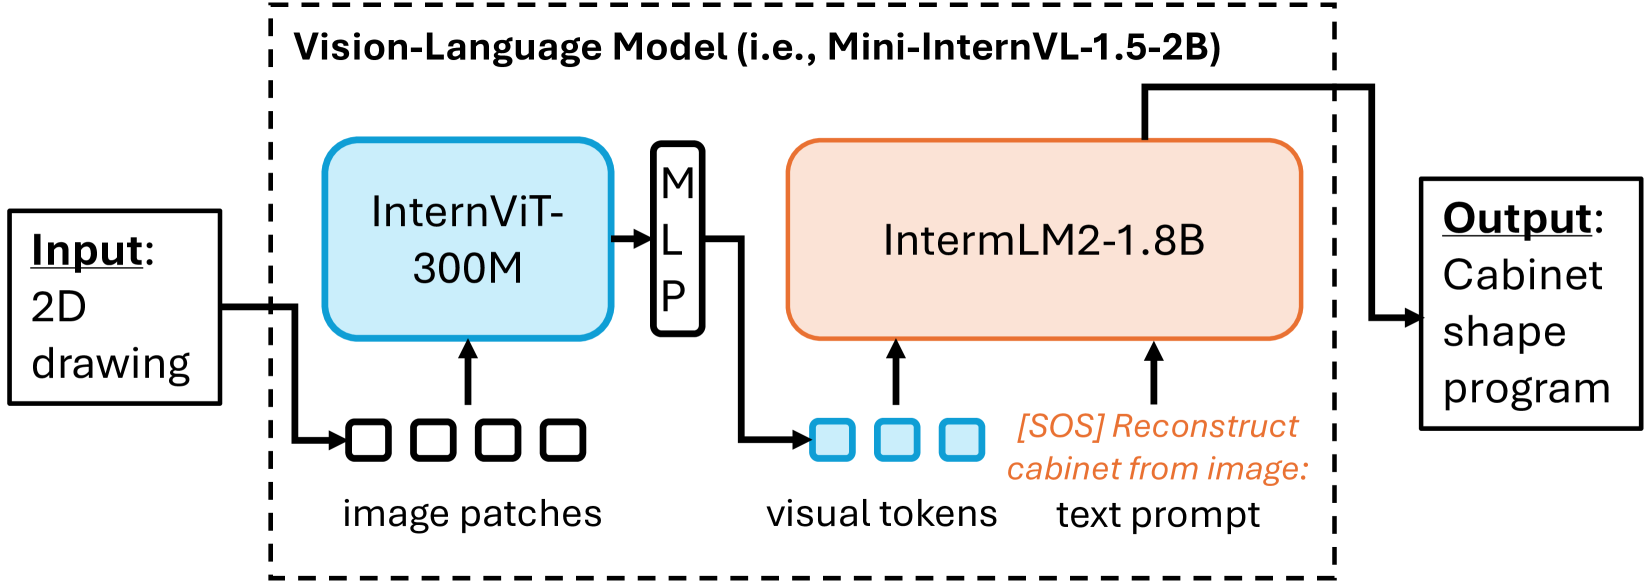
\includegraphics[width=0.9\linewidth]{internvl.png}
  \caption{High-level multimodal architecture (reference figure in repo).}
\end{figure}

\section{Repository Updates in D1.2}
\subsection{Synthetic Dataset Generator}
We added `preprocessing/generate_synthetic.py` that renders rectangles, circles, and line segments with basic dimension labels and produces aligned JSON annotations. It also writes train/val/test splits.

\subsection{Visualization and Evaluation}
`preprocessing/visualize_annotations.py` overlays bounding boxes and labels on top of images. `evaluation/metrics.py` provides IoU; `evaluation/evaluate_synthetic.py` prints simple corpus stats per split.

\subsection{Documentation}
`README.md` now includes a Quickstart showing how to generate a small dataset, visualize a sample, and get stats.

\section{Quickstart (Reproducibility)}
\begin{verbatim}
python preprocessing/generate_synthetic.py --output-dir dataset/synthetic --num-samples 100
python preprocessing/visualize_annotations.py \
  --images-dir dataset/synthetic/images \
  --annotations-dir dataset/synthetic/annotations \
  --name sketch_00010 --output dataset/synthetic/vis
python evaluation/evaluate_synthetic.py \
  --annotations-dir dataset/synthetic/annotations \
  --splits dataset/synthetic/splits/train.txt
\end{verbatim}

Generated visualizations can be included in the appendix; see `docs/example.png` for style reference.

\section{Planned Work}
\begin{itemize}[leftmargin=*]
  \item Expand primitive set (arrows, dimensions-as-text tokens) and OCR integration.
  \item Train a detector baseline (ViT/DETR) on synthetic data; add metrics (precision/recall/F1).
  \item Integrate encoder--decoder path for program reconstruction; evaluate sequence accuracy.
\end{itemize}

\section*{Acknowledgments}
We thank Innopolis University for support and compute.

\end{document}


